\documentclass[a4paper]{article}

%% Language and font encodings
\usepackage[english]{babel}
\usepackage[utf8x]{inputenc}
\usepackage[T1]{fontenc}

%% Sets page size and margins
\usepackage[a4paper,top=3cm,bottom=2cm,left=3cm,right=3cm,marginparwidth=1.75cm]{geometry}

%% Useful packages
\usepackage{amsmath}
\usepackage{graphicx}
\usepackage[colorinlistoftodos]{todonotes}
\usepackage[colorlinks=true, allcolors=blue]{hyperref}

\title{Your Paper}
\author{Edgar Ivanov}

\begin{document}
	\maketitle
	
	%%\begin{abstract}
	
	%%\end{abstract}
	
	\section{Introduction}
	
	The task is to design infrastructure solution for the "Visma Services Norway" company. "Visma Services Norway" has approximately 1200 users connecting to the virtualized desktop environment and running its entire application portfolio in it for the day to day work. This document presents infrastructure solution and outlines main design considerations in mind with the redundancy.
	
	\section{Overall plan}
	Discuss the company and its needs, present drawing. can be seen on the figure \ref{fig:Diagram}
	
	\begin{figure}
		\centering
		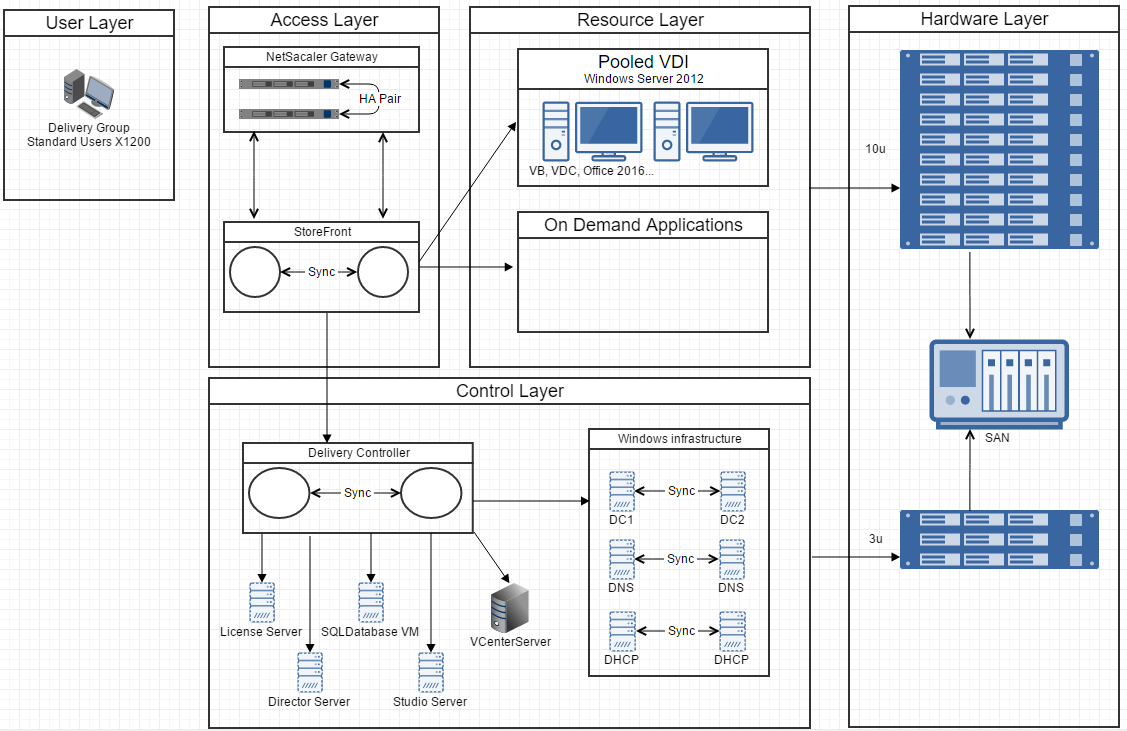
\includegraphics[width=1\textwidth]{InfrastructureDesign.png}
		\caption{\label{fig:Diagram}Infrastructure Design}
	\end{figure}
	
	\subsection{User Layer}
	Endpoint devices require Citrix Receiver to be present and correctly configured in order to access virtual desktop environment. Receiver can be deployed manually by the end users and auto configured using the provisioning file, initial deployment can also be done using GPOs or with help of any other third party solutions. Visma Services Norway (the client) is responsible for the endpoint selection and management. Client should have redundant internet connection to eliminate single point of failure in connecting to the solution.
	\subsection{Access Layer}
	
	To ensure high availability multi-active data centre deployment will be used. A pair of the VPX based NetScaler Gateways will be deployed in the DMZ zone of each delivery site. Both datacentres will have two StoreFron servers, one accepting all connections and the second one in the stand by mode for the redundancy.    
	
	\subsection{Resource Layer}
	
	VDI images should be stored on the networked storage instead of the local to eliminate image loss in case of the local disk failure. To ensure fast application provisioning all applications will be pre-installed on the base image. Non standard applications may be streamed to the user Virtual Desktops in cases where there are special requirements. For the users who need Desktop customization profiles may be saved on the DFS network share, otherwise all Desktops will be reset to the clean state.
	
	\subsection{Control Layer}
	
	All Windows components, on which Ctrix relies for the successfully application delivery, will be configured with the redundancies. There will be two Domain Controllers in each delivery site, two DNS servers as well as DHCP server configured as a cluster.
	
	Delivery controller redundancy will be achieved by having at least two of them on the different physical hosts. Each Virtual Delivery Agent will be configured with the list of the available Delivery Controllers, thus providing redundancy in case of the Delivery Controller failure. \todo{Best practice would be to utilize NetSalers HA ability}
	
	Different techniques may be employed to achieve site database redundancy such as  SQL mirroring, AlwaysOn Failover Clustering or AlwaysOn Availability Group. Having SQL database running off the shared storage in the virtual machine would allow the use of the VMWares VMotion technology, which would bring up the database on the healthy physical host sharing the same storage group. Further protection may be achieved by the use of the VSpheres replication technology with enabled quisicing, this would allow quick VM restoration in to the consistent state.
	
	Licensing server may be left over as the built 30-day grace period gives plenty of time for the service restoration.
	
	VPS high availability? No idea.         
	
	\subsection{Hardware Layer}
	
	As per the original task we know that the hosting company utilizes SAN which most likely will be running in some king of the RAID configuration, thus providing redundancy at the storage level. All other components like redundant network links, power supplies, server chassis are defacto standard. Further hardware redundancy may be achieved with the help of the VMware HA feature, which would bring up guest VMs on the different physical host in the case of the original host failure, the same approach as we have employed for the site database redundancy.
	
	Hawing initial user numbers and their usage patterns following was identified as a hardware requirement. Citrix Project Accelerator has been used in  
	
	\section{Bussiness Process}
	
	\begin{figure}
		\centering
		\includegraphics[width=1\textwidth]{VismaWorkflow.png}
		\caption{\label{fig:VismaWorkflow}Workflow Design}
	\end{figure}
	
	\subsection{How to add Citations and a References List}
	\href{https://www.citrix.com/blogs/2014/04/09/activeactive-gslb-for-xendesktop-a-practical-approach-part-1/}{Active/Active GSLB for XenDesktop}
	\href{https://www.citrix.com/blogs/2012/11/24/xendesktop-high-availability-load-balancing-add-on-for-web-interface/}{XenDesktop – High Availability \& Load Balancing Add On For Web Interface}

	
	We hope you find Overleaf useful, and please let us know if you have any feedback using the help menu above --- or use the contact form at \url{https://www.overleaf.com/contact}!
	
	\bibliographystyle{alpha}
	\bibliography{sample}
	
\end{document}